\section{Условие}

В банк приходят клиенты каждые 3$\pm$2 минуты. Если оба терминала заняты, то клиенту будет отказано. На каждом терминале происходит получение очереди за 4$\pm$3 минуты. С вероятностью 10\% в отделении банка нет необходимой услуги, тогда клиенту будет отказано. Если в очереди на окно уже 5 клиентов, клиенту отказывают. Всего есть 5 окон, которые работают 10±5, 15$\pm$5, 15$\pm$10, 20$\pm$10 и 20$\pm$5 минут соотвественно по разным услугам. Окно на терминале выбирается по равномерному распределению. После оформления бумаг в окнах 1 и 2, с клиентом идут в кабинет для оформления кредита, который оформляется 10$\pm$5 минут. С вероятностью 5\% в окне не могут помочь клиенту, тогда ему отказывают. Промоделировать процесс обработки 500 клиентов. Определить вероятность отказа.

\section{Теория}

На рисунке \ref{fig:model} представлена структурная схема  данной концептуальной модели.

\begin{figure}[H]
    \centering
    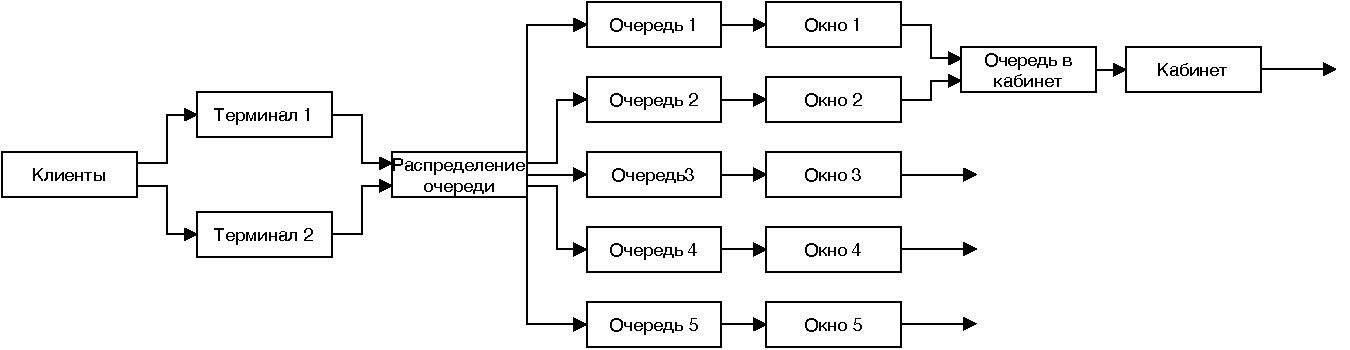
\includegraphics[width=0.9\textwidth]{img/content/model.pdf}
    \caption{Структурная схема}
    \label{fig:model}
\end{figure}

Поскольку значение требующейся в условии вероятности отказа находится в промежутке, то необходимо смоделировать систему много раз.

\section{Результаты}

На рисунке \ref{fig:result} представлен результат полученный путем 1000 моделирований системы.

\begin{figure}[H]
    \centering
    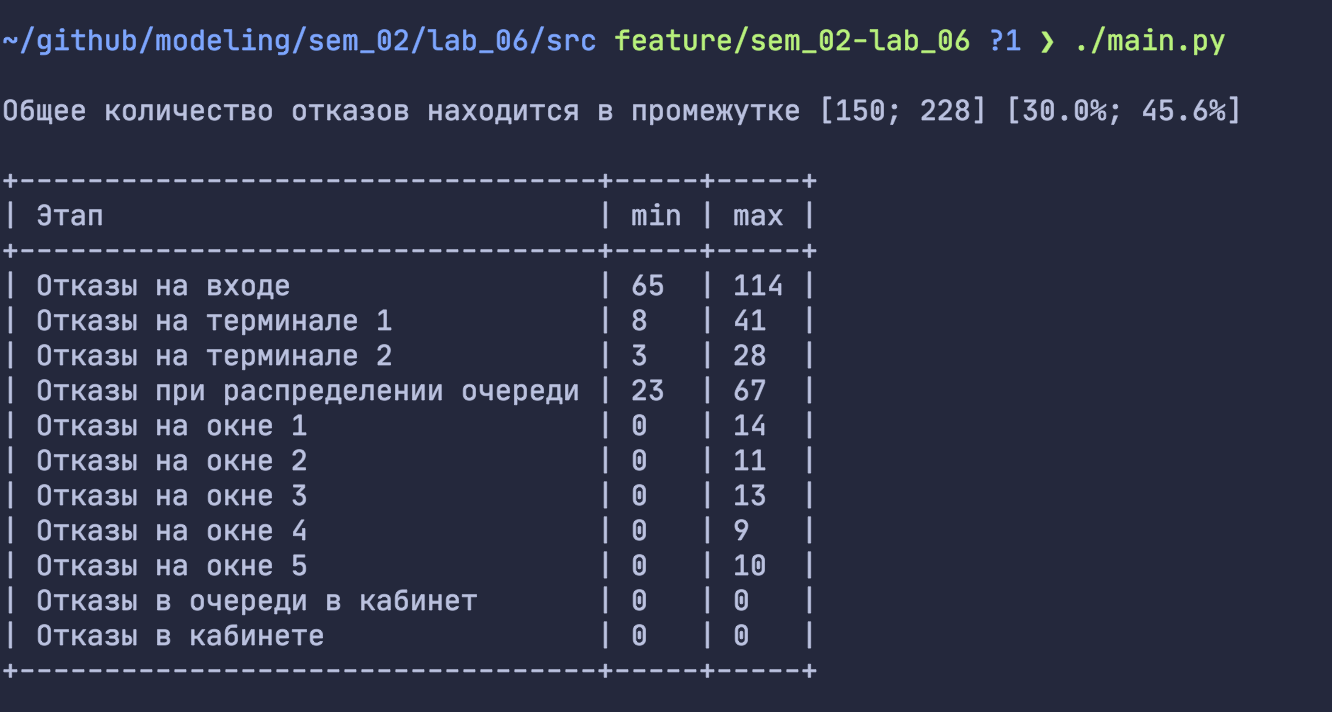
\includegraphics[width=0.8\textwidth]{img/content/result.png}
    \caption{Полученный результат}
    \label{fig:result}
\end{figure}

Исходя из результата видно, что к комнате и очереди на комнату никогда не было отказов, поскольку очередь туда не предусматривает ограничений и нет вероятности отказа. Так же из-за низкой вероятности отказа в окнах были ситуации, при которых не было ни одного отказа.

\section{Вывод}

Разработана программа, результатом работы которой являются промежутки, в которых находились значения вероятности отказа и количества отказов на каждом этапе, полученных в результате 1000 моделирований системы работы банка.
